%!TEX root = ../../../../memoria.tex
\subsection{\paymentsCOM}\label{cap:solucionImplementada:section:dashboard:subsection:payment}
	En establecimientos tradicionales \brickandmortar, un cliente ve un producto, lo examina, y entonces paga utlizando dinero, cheques, o tarjetas de crédito.
	% In traditional brick-and-mortar establishments, a customer sees a product, examines
	% it, and then pays for it by cash, check, or credit card (see Figure 6-1).

	En el mundo \ecommerceCOM, en la mayoría de los casos un cliente no ve físicamente el producto al momento de realizar la transacción, y el método de pago es realizado electrónicamente. Por lo tanto, temas de confianza y aceptación juegan un rol más importante en el mundo \ecommerceCOM que en el mundo de negocios tradicionales en lo que a sistemas de pago se refiere \cite{bidgoli2002electronic}.
	% In the e-commerce world, in most cases the customer does not physically see
	% the actual product at the time of transaction, and the method of payment is performed
	% electronically. Therefore, issues of trust and acceptance play a more important
	% role in the e-commerce world than in traditional businesses as far as payment
	% systems are concerned.

	Los sistemas de pago electrónico (\epsSiglasCOM, siglas en inglés) utilizan \hardwarePC y \softwarePC que permiten a los clientes pagar por productos y servicios en línea. Aunque estos sistemas podrían ser considerados inmaduros por los más críticos, no puede negarse el constante avance que viven periódicamente. El principal objetivo de un \epsSiglasCOM son incrementar eficiencia, mejorar seguridad, y lograr una mayor comodidad y facilidad de uso para los clientes \cite{bidgoli2002electronic}.
	% EPSs utilize integrated hardware and software systems that enable a customer
	% to pay for the goods and services online. Although these systems are in their infancy,
	% some significant progress has been made. The main objectives of EPS are
	% to increase efficiency, improve security, and enhance customer convenience and
	% ease of use. As shown throughout this chapter, there are several methods and
	% instruments that can be used to enable EPS implementation (see Figure
	% 6-2.)

	%Provide a Number of Payment Methods
	% 	It sounds obvious, but there are websites that offer only one payment method. However, data highlighted in an infographic from Milo shows that 56% of respondents expect a variety of payment options on the checkout page.
	Es importante agregar varios métodos de \paymentsCOM. Puede sonar obvio, pero existen métodos que aún ofrecen solo una manera de realizar un pago. Un estudio demuestra que el 56\% de usuarios espera una variedad de opciones de \paymentsCOM en la página de \checkoutCOM \cite{online_kissmetrics_easy_payment_process}.

	% While it’s not necessary – nor practical for that matter – to offer every conceivable payment method available, you’ll want to take a look at your target audience to see which payment methods they use.
	Aunque en la práctica es innecesario e impracticable ofrecer todos los métodos de pagos existentes, se deseará observar la preferencia del público para determinar cuáles son los métodos que ellos utilizan. Entonces se agregarán aquellos para capturar a la mayoría de los visitantes al \websiteINT \cite{online_kissmetrics_easy_payment_process}.

	En el contexto de esta memoria, solo se implementará \paypalNAME como servicio de pago.
	
	\subsubsection{\paypalNAME}

		\paypalNAME es un servicio global que mueve los montos de pago desde una tarjeta de crédito hacia el vendedor sin compartir la información financiera. \paypalNAME ofrece una variedad de productos y soluciones para aceptar pagos. De estos uno ha sido elegido para permitir el flujo completo de compra, pero siempre considerando la opción de agregar nuevos métodos en un futuro.

		% TODO: ver si alcanzo agregar el otro método
		%De estos, se han elegido dos los cuales han sido considerados adecuados para los requerimientos.

		%PayPal is a global service that moves the payment amount from your credit card to the merchant without sharing your financial information. %PayPal offers a variety of products and solutions for accepting payments. You can choose the solution that is best for your requirements, whether your goal is to get up and running as quickly as possible or to develop a fully customized payment experience.

		\subsection*{\PPPaymentProNAME}\label{chapter:solucionImplementada:dashboard:payment:subsection:paypal_pro}
			\PPPaymentProNAME es una solución customizable que permite a los vendedores mantener a los compradores dentro de su \websiteINT durante el proceso completo de \paymentsCOM y \checkoutCOM. Los vendedores pueden mantener sus propios sitios de \checkoutCOM personalizados y enviar transacciones a \paypalNAME, o es posible también tener un \hostCPT de \paypalNAME que tenga páginas de \checkoutCOM e incluso manejar la seguridad para las ventas y autorización. \PPPaymentProNAME puede aceptar pagos de \paypalNAME y  \paypalCreditNAME, al igual que con tarjetas de crédito de pago \cite{online_paypal_developer_acceptpayments}.
			% PayPal Payments Pro is a customizable solution that enables merchants to keep buyers on their website during the entire checkout and payment process. Merchants can host their own customized checkout pages and send transactions to PayPal, or they can have PayPal host the checkout pages and also manage security for sales and authorizations. PayPal Payments Pro can accept Paypal and PayPal credit payments, as well as credit and debit card payments. PayPal Payments Pro also includes an optimized mobile checkout experience. For details, see PayPal Payments Pro.

			Para el uso de este servicio, es necesaria la creación de una \paypalNAME \appINT. Toda la información necesaria se encuentra en la documentación para los desarrolladores \cite{online_paypal_developer_apps_credentials}, pero en resumen, lo relevante acá para lograr una configuración adecuada son 3 elementos:

				\begin{itemize}
					\item Existen dos ambientes de trabajo: \sandboxEnvPL y \liveEnvPL.
					\item \clientIDPayPal.
					\item \secretPayPal.
				\end{itemize}

			Tanto el \clientIDPayPal como el \secretPayPal dependen del ambiente en el cual me encuentro.

			Desde el \dashboardEF es posible acceder al menú configurable de \paypalNAME, el cual permite agregar esta información (ver \refFigura{figure:payment:paypal:payflow_pro:form}).

			\begin{figure}[H]
				\centering
				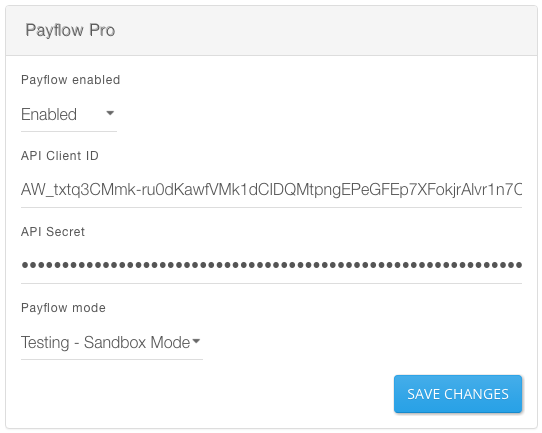
\includegraphics[width=0.8\textwidth]{figuras/payment/form.png}
				\caption{Formulario para agregar la configuración necesaria para el uso de \paypalPayFlowNAME.}
				\label{figure:payment:paypal:payflow_pro:form}
			\end{figure}

			El formulario de \paypalNAME se somete a las restricciones visibles en la \refTabla{tab:payment:paypal:payflow_pro:form}.

			\begin{table}[H]
			    \centering
				\begin{tabular}{ |l|c||l| }
					\hline Campo & Requerido & Restricción \\ \hline
					\multirow{1}{*}{\textit{Payflow enabled}} 	&  \checkmark 	& Boolean.\\ \hline
					\multirow{1}{*}{\textit{Client ID}} 		&  				& \\ \hline
					\multirow{1}{*}{\textit{Secret}} 			&  				& \\ \hline
					\multirow{1}{*}{\textit{PayFlow Mode}} 		&  \checkmark	& Boolean.\\ \hline
					\hline
				\end{tabular}
			 	\caption{ Resumen restricciones formulario \paypalPayFlowNAME.}
			    \label{tab:payment:paypal:payflow_pro:form}
			\end{table}
			
